\begin{figure}[H] \centering
\subsection{BDD (SK)}
{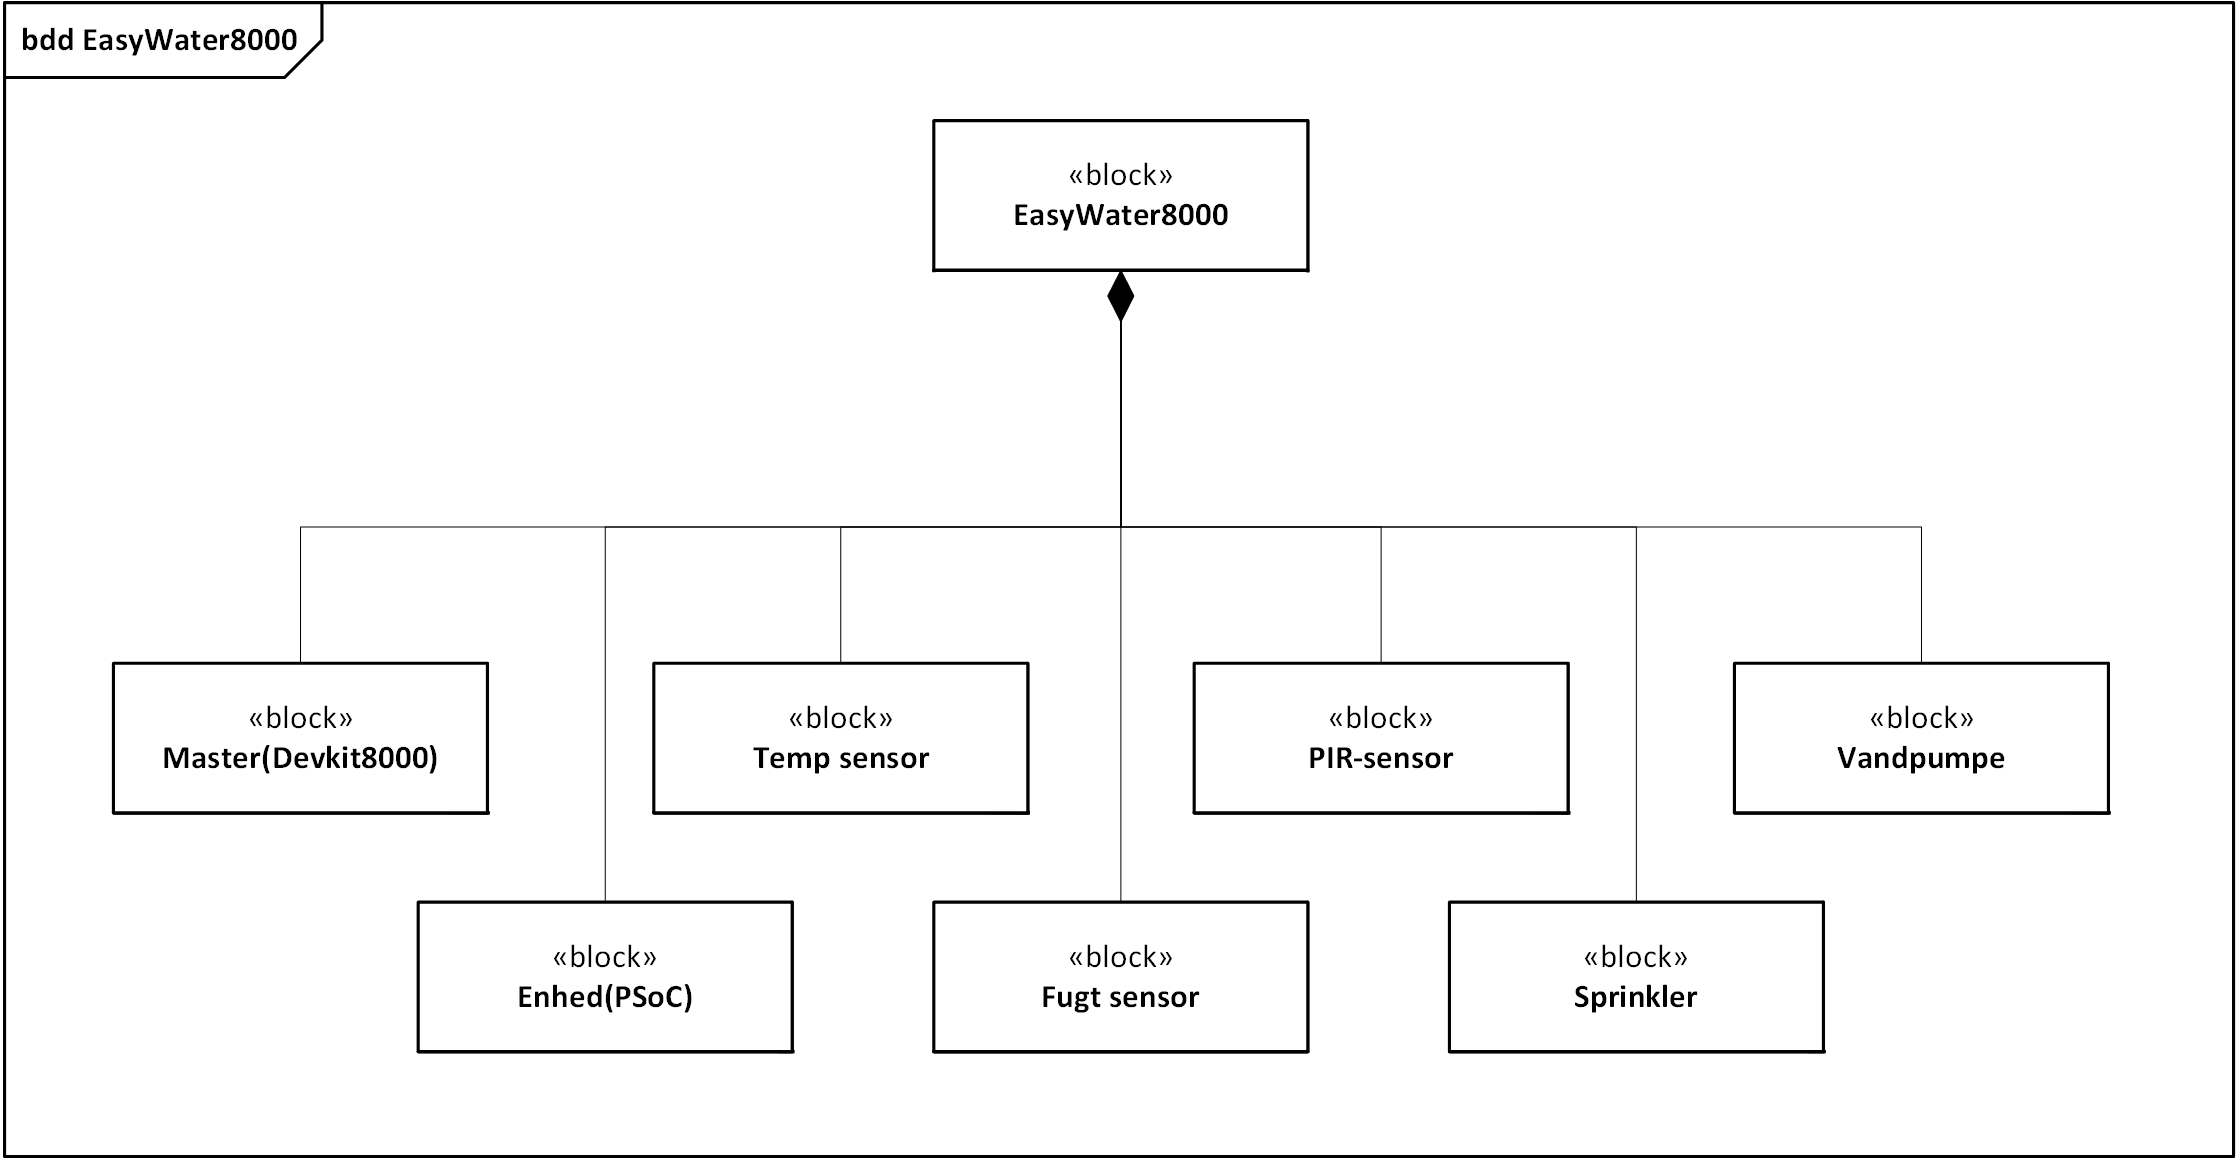
\includegraphics[width=0.9\textwidth]{filer/systemarkitektur/BDD}}
\caption{BDD}
\label{lab:bdd}
\raggedright
\end{figure}
BDD diagrammet giver et overblik over hvad det samlede system består af. \newline \newline
\textbf{Master(Devkit8000)}: Devkit8000 er master der styrer hele systemet, den modtager inputs fra en touchskærm.  \newline \newline
\textbf{Enhed(PSoC)}: PSoC'en er grænsefladen til den fysiske verden, den indsamler data fra sensorer. Den modtager ordre fra devkit8000 der styrer hvad der skal ske. 		\newline \newline
\textbf{Temperatursensor}: Har til opgave at indsamle temperaturmålinger. \newline \newline
\textbf{Fugtsensor}: Har til opgave at indsamle fugtighedsmålinger. \newline \newline
\textbf{PIR-sensor}: Har til opgave at detektere om der er bevægelse på banen. \newline \newline
\textbf{Sprinkler}: Har til opgave at sprede vand ud på banen. \newline \newline
\textbf{Vandpumpe}: Har til opgave at forsyne sprinkleren med vand. \newline \newline

\begin{figure}[H] \centering
\subsection{BDD Master (MK)}
{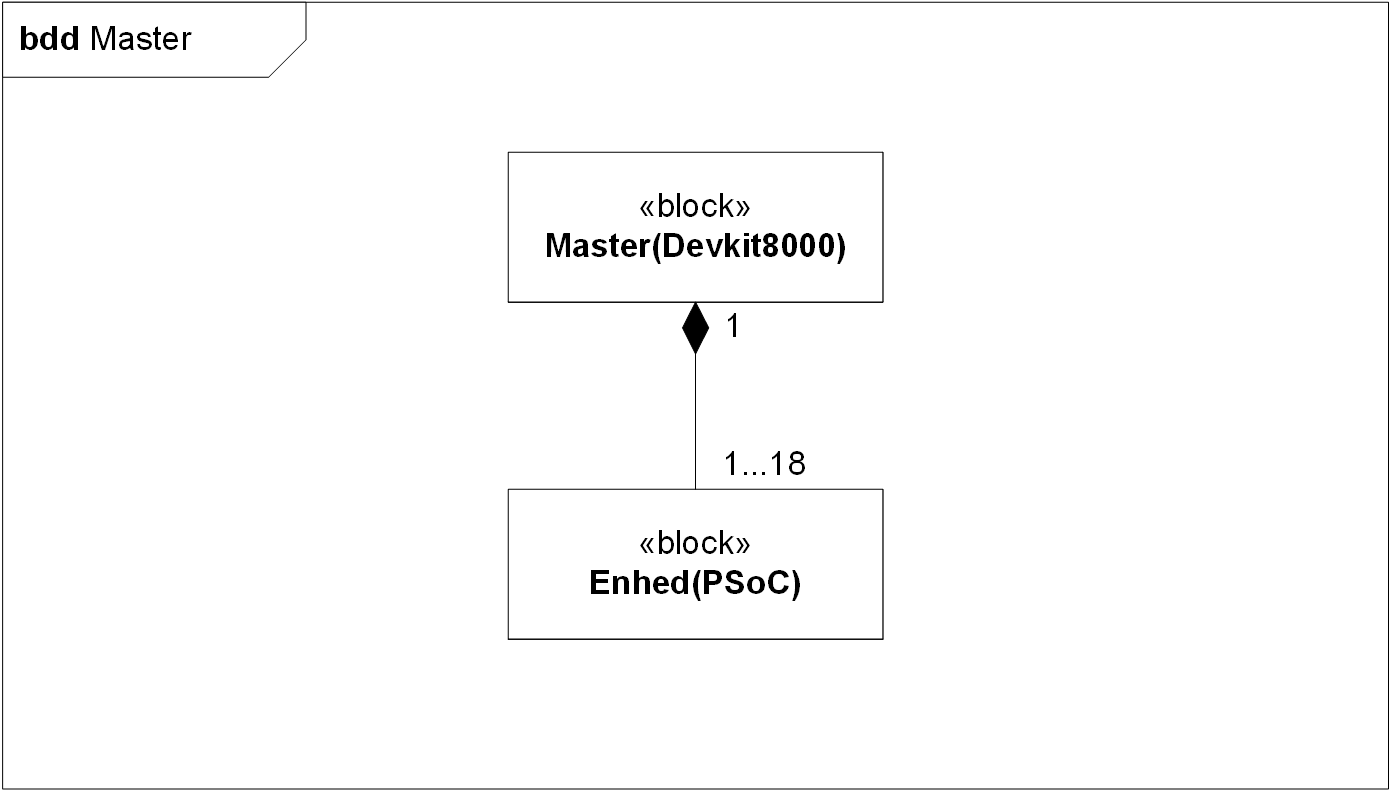
\includegraphics[width=0.9\textwidth]{filer/systemarkitektur/BDD_Master}}
\caption{BDD Master}
\label{lab:bddmaster}
\raggedright
\end{figure}
BDD diagrammet giver et overblik over hvad Master består af.

\begin{figure}[H] \centering
\subsection{BDD Enhed (MK)}
{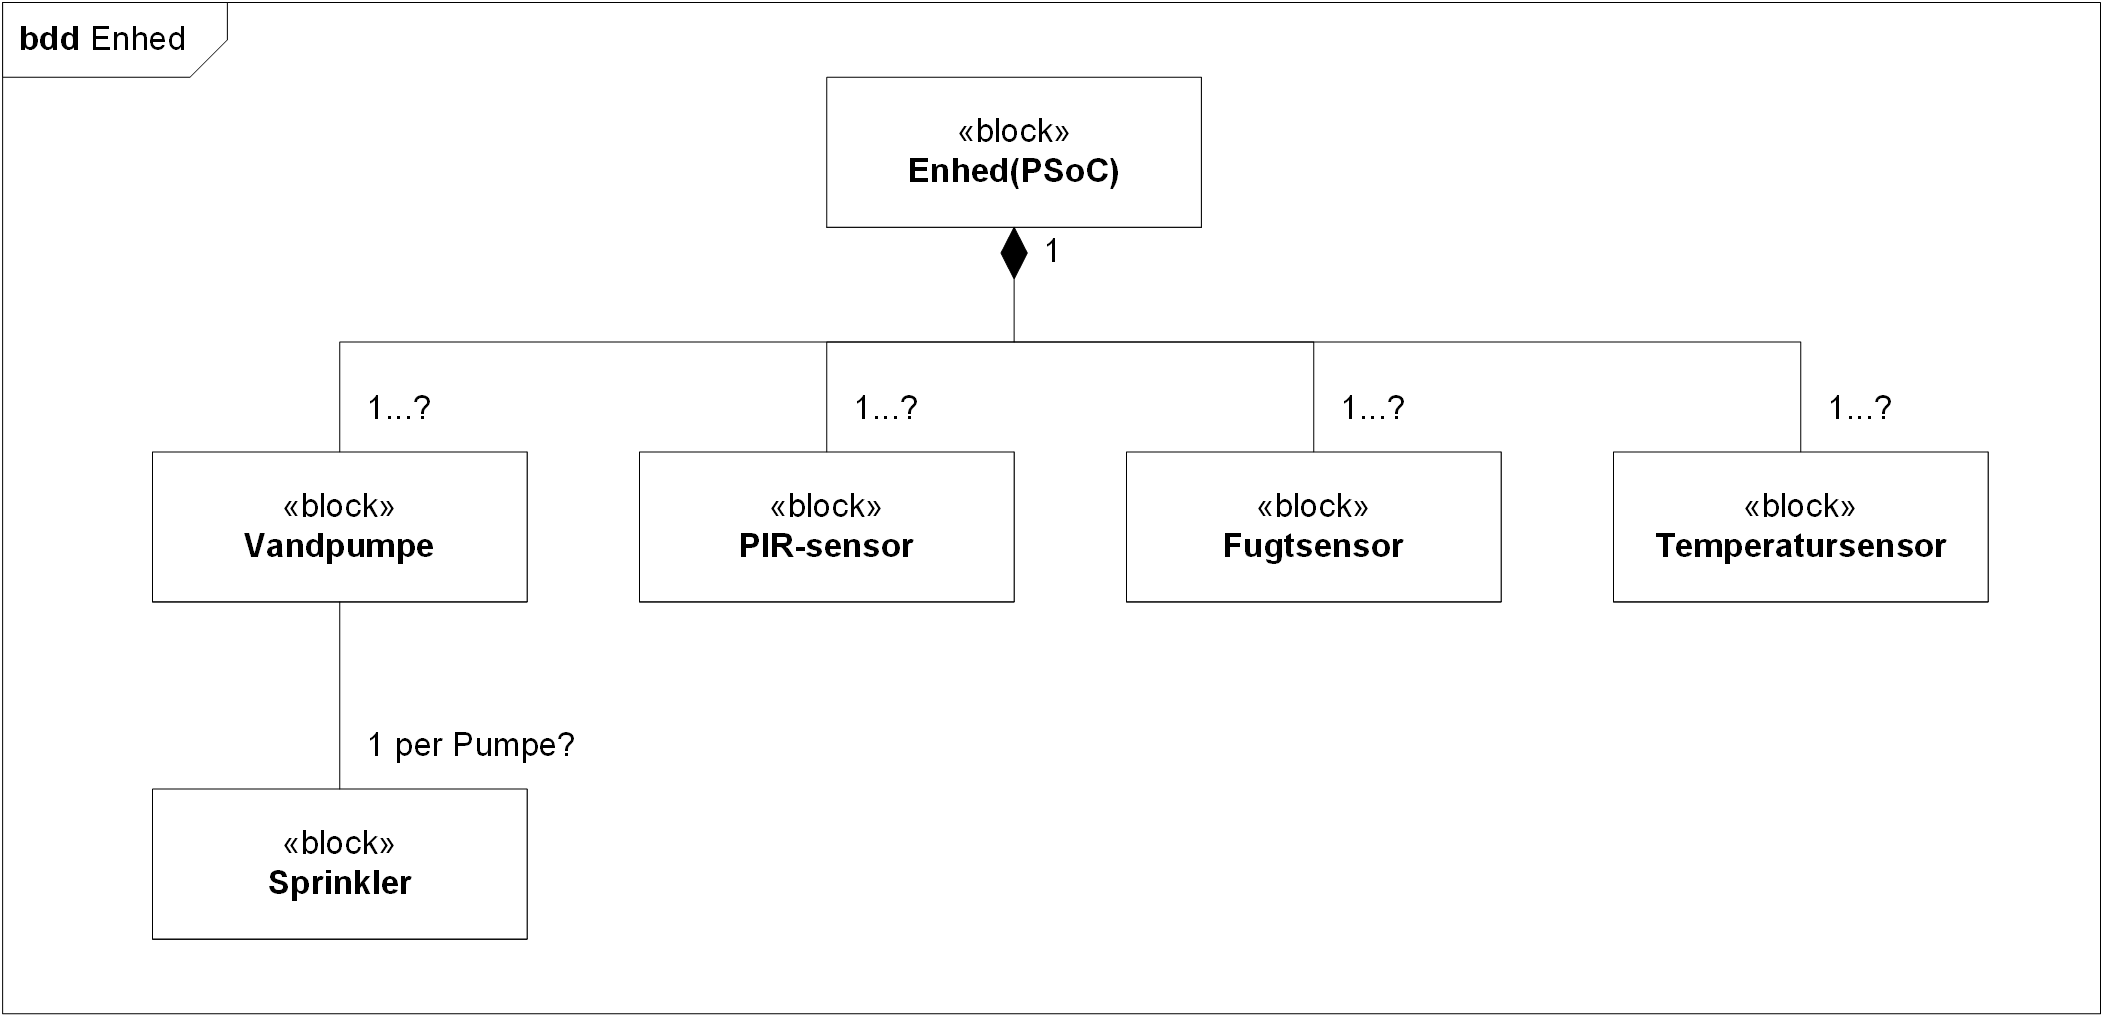
\includegraphics[width=0.9\textwidth]{filer/systemarkitektur/BDD_Enhed}}
\caption{BDD Enhed}
\label{lab:bddenhed}
\raggedright
\end{figure}
BDD diagrammet giver et overblik over hvad Enhed består af.

\begin{figure}[H] \centering
\subsection{IBD (SK)}
{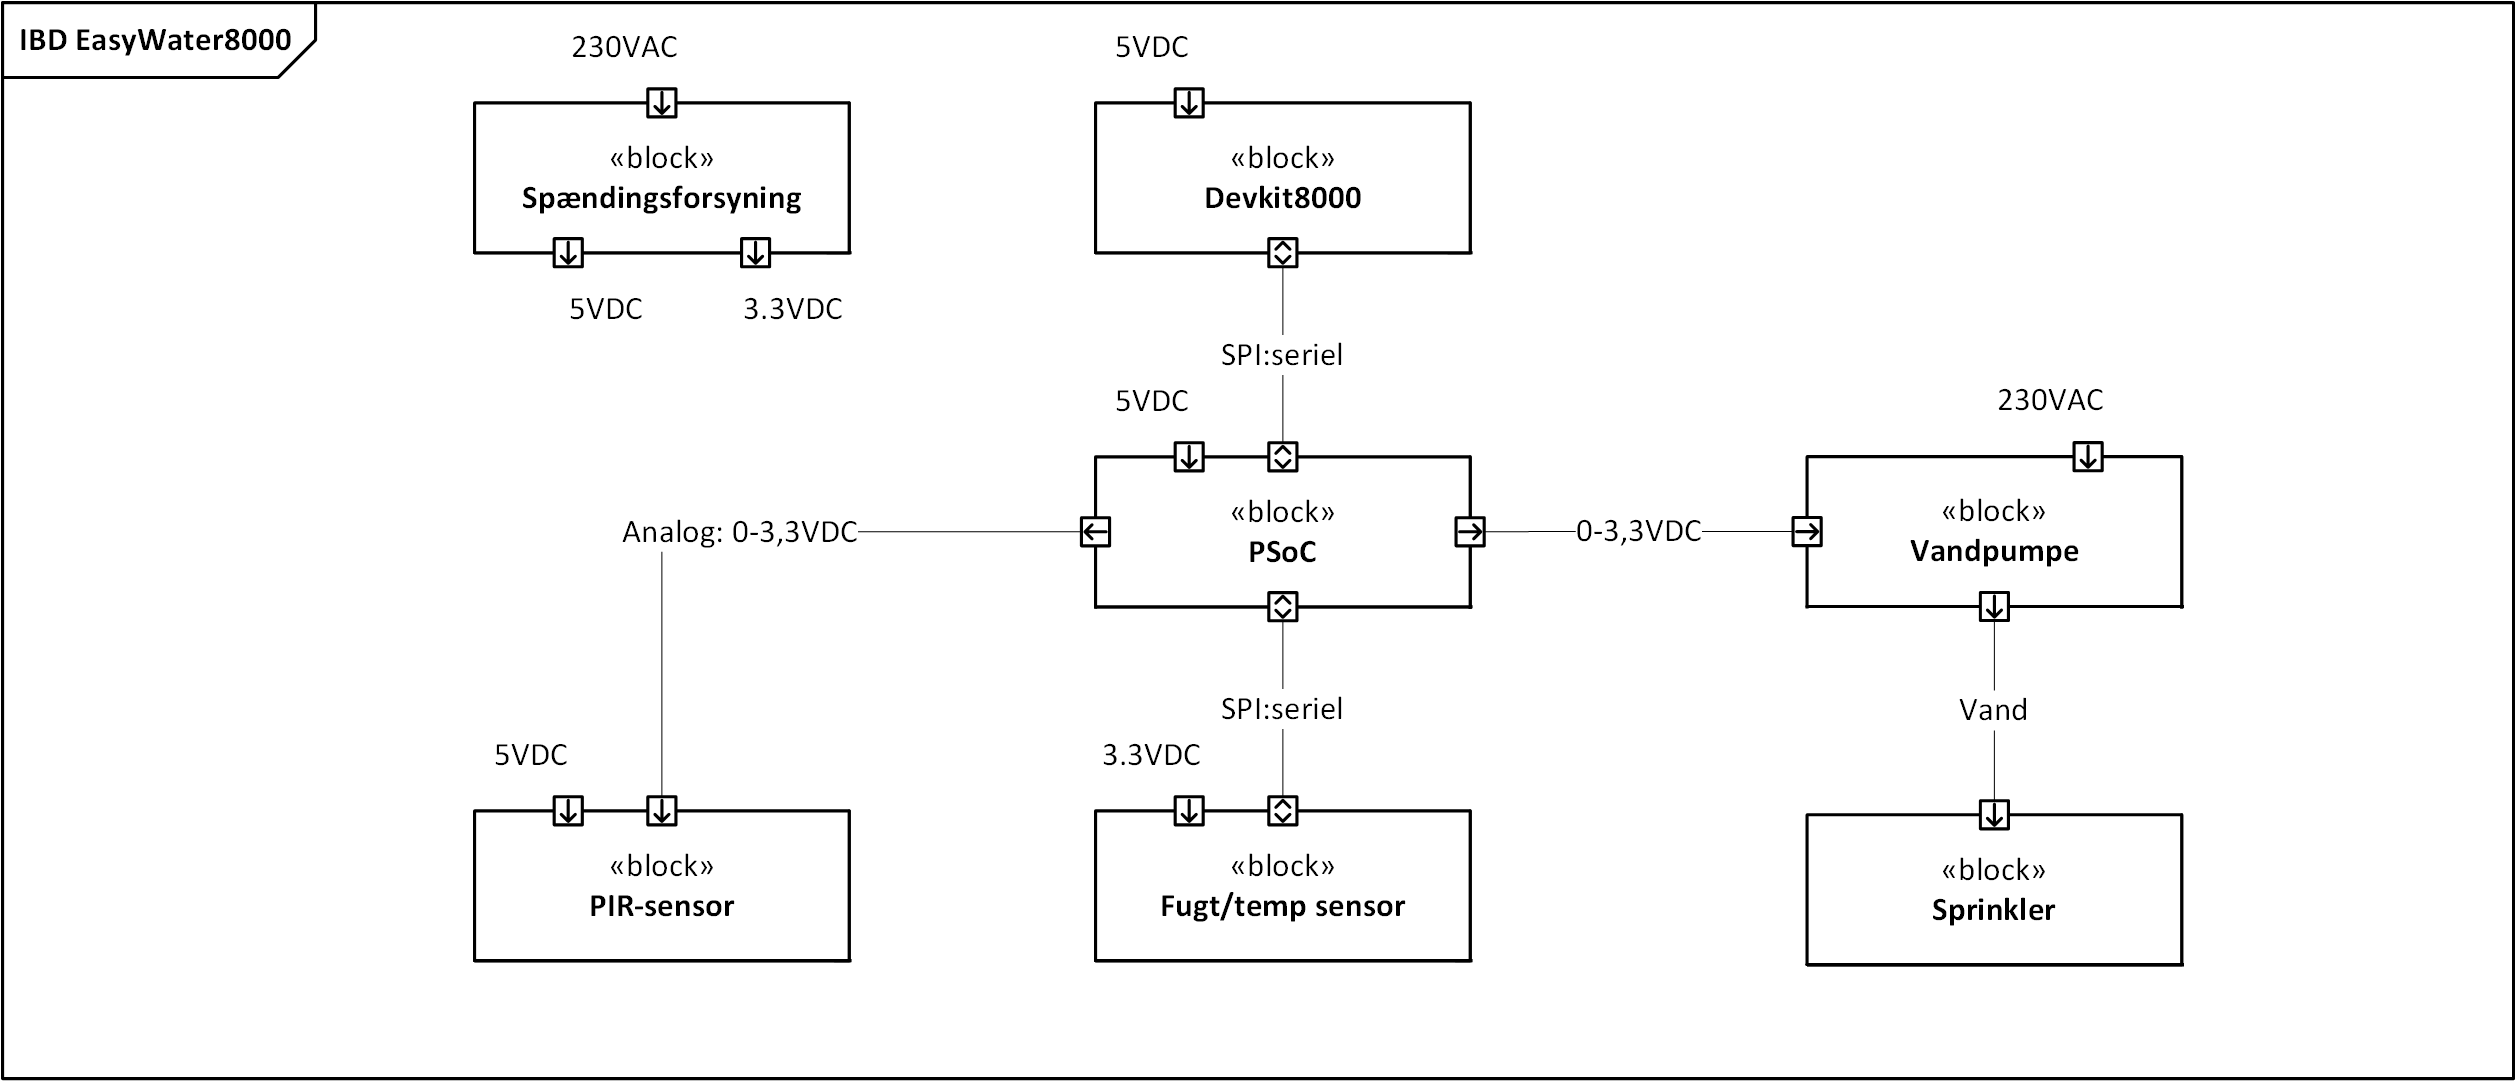
\includegraphics[width=0.9\textwidth]{filer/systemarkitektur/IBD}}
\caption{IBD}
\label{lab:ibd}
\raggedright
\end{figure}
IBD diagrammet giver et internt overblik over hvordan hele vores system er forbundet. Vi ser hvilke type signaler der bliver sendt imellem de forskellige blokke.
